\documentclass{llncs}
\usepackage{times}
\usepackage[T1]{fontenc}

% Comentar para not MAC Users
%\usepackage[applemac]{inputenc}

\usepackage{a4}
%\usepackage[margin=3cm,nohead]{geometry}
\usepackage{epstopdf}
\usepackage{indentfirst}
\usepackage{graphicx}
\usepackage{float}
\usepackage{fancyvrb}
\usepackage{amsmath}
%\renewcommand{\baselinestretch}{1.5}

\begin{document}
\mainmatter
\title{TP4: Redes Sem Fios (802.11)}

\titlerunning{TP4: Redes Sem Fios (802.11)}

\author{Diogo Braga \and João Silva \and Ricardo Caçador}

\authorrunning{Diogo Braga \and João Silva \and Ricardo Caçador}

\institute{
University of Minho, Department of  Informatics, 4710-057 Braga, Portugal\\
e-mail: \{a82547,a82005,a81064\}@alunos.uminho.pt\\
PL4, Grupo 7
}

\date{}
\bibliographystyle{splncs}

\maketitle

\section{Acesso Rádio}

\subsection{Exercício 1}
\emph{Identifique em que frequência do espectro está a operar a rede sem fios, e o canal que corresponde essa frequência.}

\begin{figure}[H]
\begin{center}
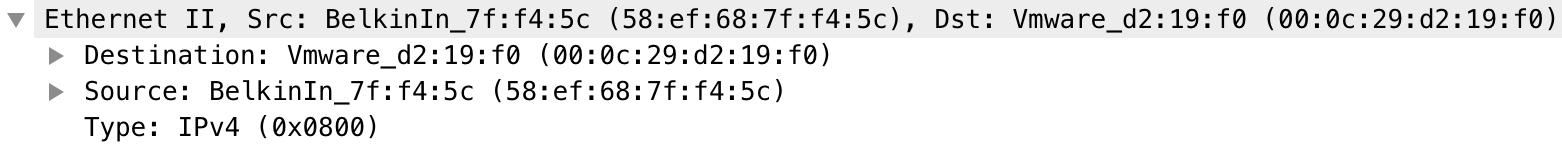
\includegraphics[scale=0.45]{1.png} 
\end{center}
\caption{\label{fig:1}802.11 Radio Information}
\end{figure} 
\par
\textbf{R:} Como se pode observar na figura \ref{fig:1} delimitado a vermelho, a rede sem fios opera na frequência \textbf{2467 MHz}, no canal \textbf{12}.


\subsection{Exercício 2}
\emph{Identifique a versão da norma IEEE 802.11 que está a ser usada.}
\\ \par
\textbf{R:} A versão usada é a \textbf{802.11g}. Tal pode ser verificado sublinhado a azul na \ref{fig:1}.


\subsection{Exercício 3}
\emph{Qual o débito a que foi enviada a trama escolhida? Será que esse débito corresponde ao débito máximo a que a interface WiFi pode operar? Justifique.}
\\ \par
\textbf{R:} A trama foi enviada a um débito de \textbf{1.0 Mb/s}, como se pode verificar na \ref{fig:1} sublinhado a verde. Este débito não corresponde ao máximo que a interface Wifi pode operar, pois segundo a norma 802.11g é oferecida uma velocidade máxima de 54 Mb/s.


\section{Scanning Passivo e Scanning Ativo}

\subsection{Exercício 4}
\emph{Selecione uma trama beacon (e.g., a trama 3XX). Esta trama pertence a que tipo de tramas 802.11? Indique o valor dos seus identificadores de tipo e de subtipo. Em que parte concreta do cabeçalho da trama estão especificados (ver anexo)?}

\begin{figure}[H]
\begin{center}
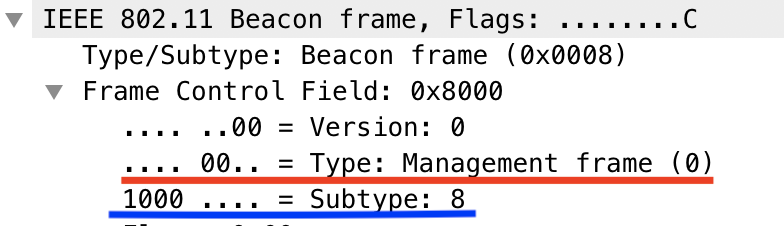
\includegraphics[scale=0.45]{4.png} 
\end{center}
\caption{\label{fig:4}Tipo e Subtipo da Trama}
\end{figure} 
\par
\textbf{R:} Esta trama é do tipo \textbf{Management}, e valor que o identifica é o \textbf{0}, como sublinhado na \ref{fig:4} a vermelho. O subtipo da trama é \textbf{Beacon}, e o valor que o identifica é o \textbf{8}, em binário \textbf{1000}. Estes valores estão especificados no byte 26 do cabeçalho da trama.

\subsection{Exercício 5}
\emph{Liste todos os SSIDs dos APs (Access Points) que estão a operar na vizinhança da STA de captura? Explicite o modo como obteve essa informação. Como sugestão pode construir um filtro de visualização o apropriado (tomando como base a resposta da alínea anterior) que lhe permita obter a listagem pretendida.}

\begin{figure}[H]
\begin{center}
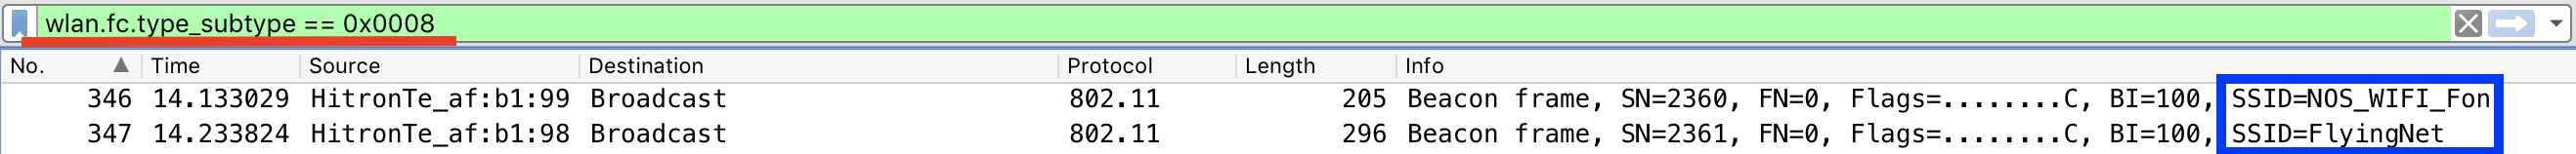
\includegraphics[scale=0.30]{5.png} 
\end{center}
\caption{\label{fig:5}Diferentes SSID.}
\end{figure} 
\par
\textbf{R:} Como se pode observar na figura \ref{fig:5} delimitado a azul, os dois SSIDs dos Access Points que estão a operar na vizinhança da STA de captura são o \textbf{FlyingNet} e o \textbf{NOS\_WIFI\_Fon}. Todas as restantes tramas Beacon presentes na captura pretencem a estes dois SSIDs. Tal foi mais facilmente obtido usando o filtro de visualização \textbf{wlan.fc.type\_subtype == 0x0008} sublinhado a vermelho na figura. Este comando filtra todos os subtipos que são Beacon.


\subsection{Exercício 6}
\emph{Verifique se está a ser usado o método de detecção de erros (CRC), e se todas as tramas Beacon são recebidas corretamente. Justifique o porquê de usar detecção de erros neste tipo de redes locais.}
\begin{figure}[H]
\begin{center}
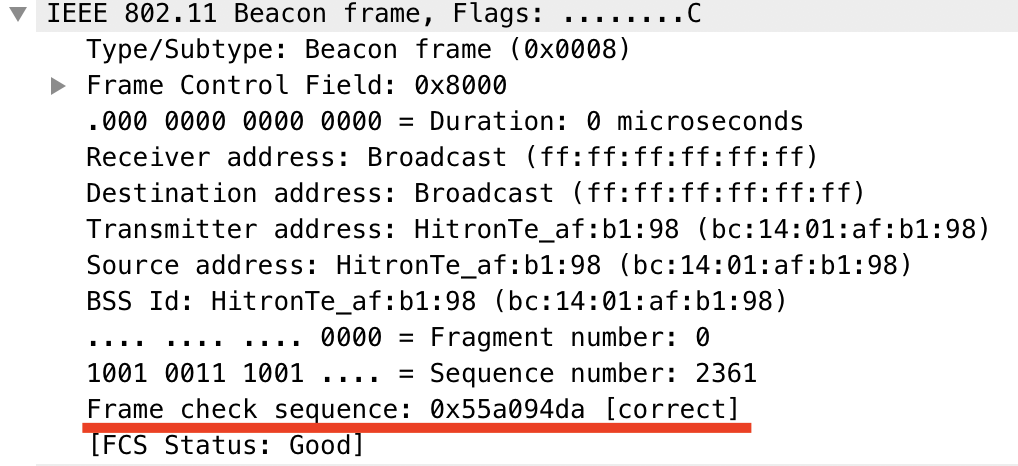
\includegraphics[scale=0.30]{6.png} 
\end{center}
\caption{\label{fig:6} Campo CRC.}
\end{figure} 

\begin{figure}[H]
\begin{center}
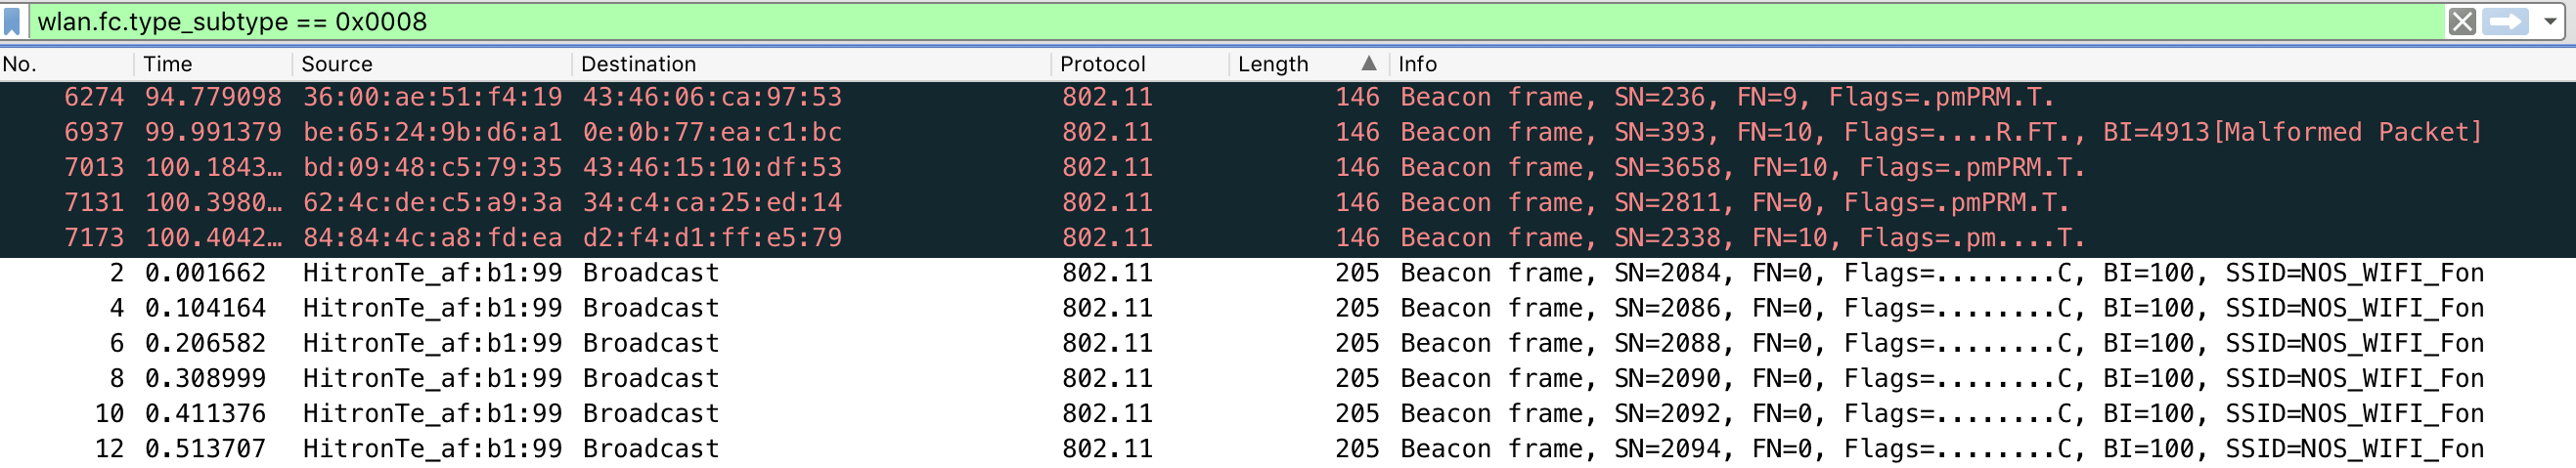
\includegraphics[scale=0.30]{6_2.png} 
\end{center}
\caption{\label{fig:6_2} Tramas Beacon com erros.}
\end{figure} 
\par
\textbf{R:} Como se pode verificar na figura \ref{fig:6} sublinhado a vermelho, está a ser usado o \textbf{Frame Check Sequence} no campo CRC. Este campo é usado para que quem recebe a trama consiga detetar erros nos bits. Num ambiente Wireless, neste caso 802.11, a existência destes erros é muito mais comum.

Como se pode constatar na figura \ref{fig:6_2}, existem 5 tramas Beacon cujo campo CRC indica a existência de erros.


\subsection{Exercício 7}
\emph{Para dois dos APs identificados, indique qual é o intervalo de tempo previsto entre tramas beacon consecutivas? (Nota: este valor é anunciado na própria trama beacon). Na prática, a periodicidade de tramas beacon é verificada? Tente explicar porquê.}
\begin{figure}[H]
\begin{center}
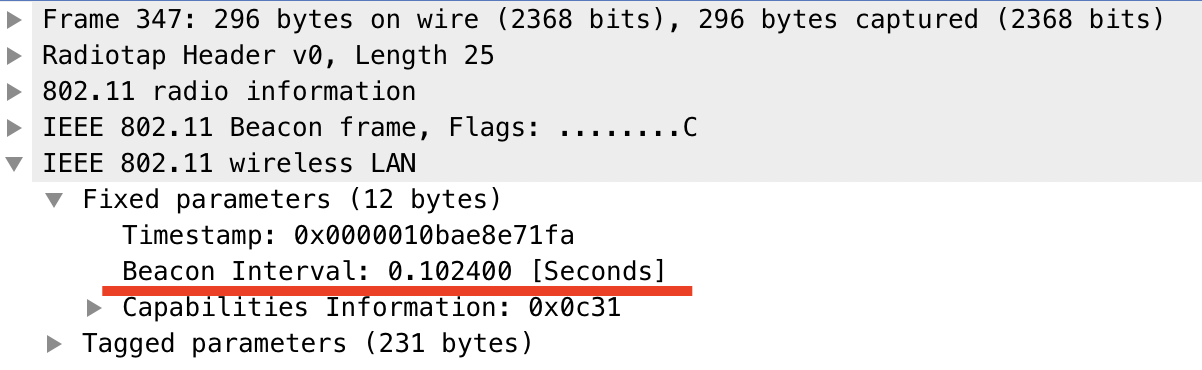
\includegraphics[scale=0.30]{7_347.png} 
\end{center}
\caption{\label{fig:7_347} Beacon Interval da trama 347.}
\end{figure} 
\par
\begin{figure}[H]
\begin{center}
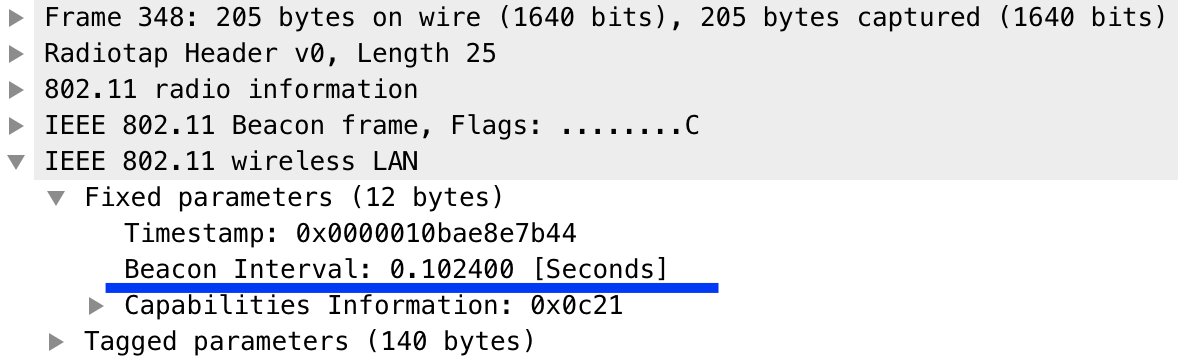
\includegraphics[scale=0.30]{7_348.png} 
\end{center}
\caption{\label{fig:7_348}Beacon Interval da trama 348.}
\end{figure} 

\begin{figure}[H]
\begin{center}
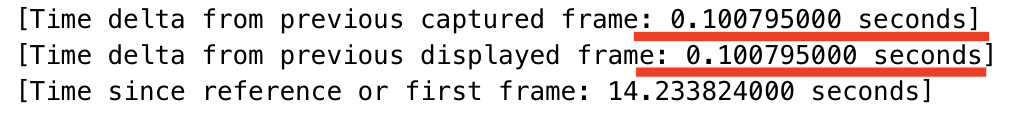
\includegraphics[scale=0.30]{7_2.png} 
\end{center}
\caption{\label{fig:7_2}Tempo entre tramas.}
\end{figure} 
\par
\textbf{R:} Como se pode verificar na figura \ref{fig:7_347} sublinhado a vermelho, o intervalo de tempo previsto para a trama 347 é \textbf{0.102400 s}. Para a trama 348 o intervalo de tempo previsto é também \textbf{0.102400 s}, tal como pode ser verificado sublinhado a azul na \ref{fig:7_348}.

Analisando várias tramas nota-se que a periodicidade é verificada, pois o tempo entre tramas Beacon é muito próximo ao \textbf{Beacon Interval}, como se pode constatar na figura \ref{fig:7_2}.


\subsection{Exercício 8}
\emph{Identifique e registe todos os endereços MAC usados nas tramas beacon enviadas pelos APs. Recorde que o endereçamento está definido no cabeçalho das tramas 802.11, podendo ser utilizados até quatro endereços com diferente semântica. Para uma descrição detalhada da estrutura da trama 802.11, consulte o anexo ao enunciado.}
\begin{figure}[H]
\begin{center}
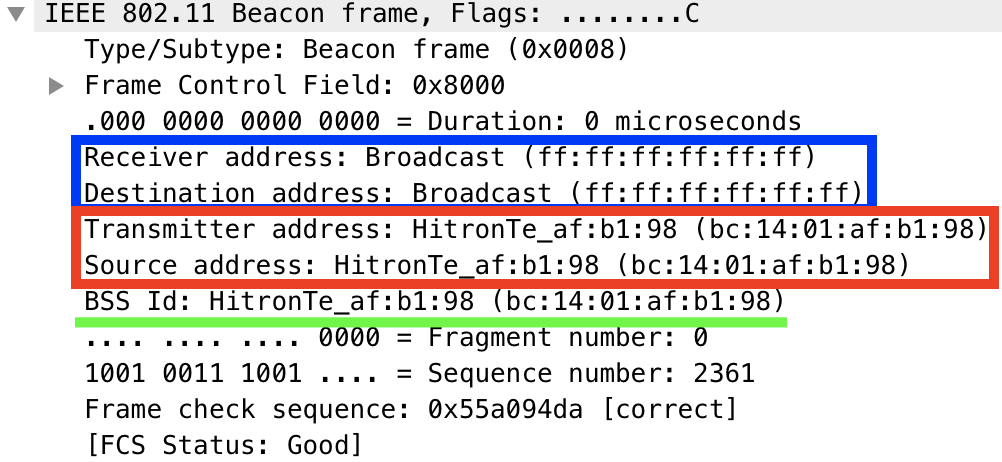
\includegraphics[scale=0.30]{8.png} 
\end{center}
\caption{\label{fig:8}Addressing de uma trama Beacon.}
\end{figure} 
\par
\textbf{R:} Como se pode observar na figura \ref{fig:8}, estamos perante 3 endereços MAC. O endereço 1 é \textbf{ff:ff:ff:ff:ff:ff}, o endereço 2 é \textbf{bc:14:01:af:b1:98}, e o endereço 3 é \textbf{bc:14:01:af:b1:98}. Neste caso, o endereço 4 não está a ser usado.


\subsection{Exercício 9}
\emph{As tramas beacon anunciam que o AP pode suportar vários débitos de base assim como vários "extended supported rates". Indique quais são esses débitos?}
\begin{figure}[H]
\begin{center}
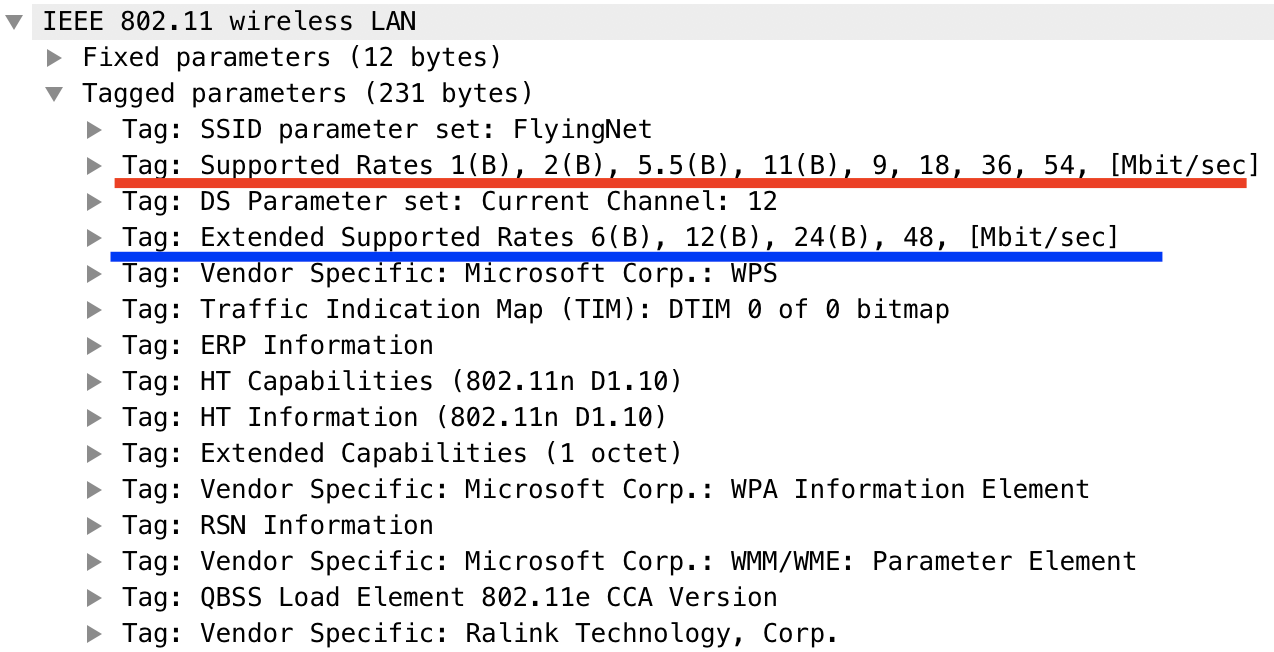
\includegraphics[scale=0.30]{9.png} 
\end{center}
\caption{\label{fig:9}Débitos Suportados.}
\end{figure} 
\par
\textbf{R:} Os débitos de base suportados encontram-se na figura \ref{fig:9} sublinhados a vermelho, enquanto os \emph{extended supported rates} se encontram sublinhados a azul.


\subsection{Exercício 10}
\emph{Estabeleça um filtro Wireshark apropriado que lhe permita visualizar todas as tramas probing request ou probing response, simultaneamente.}
\begin{figure}[H]
\begin{center}
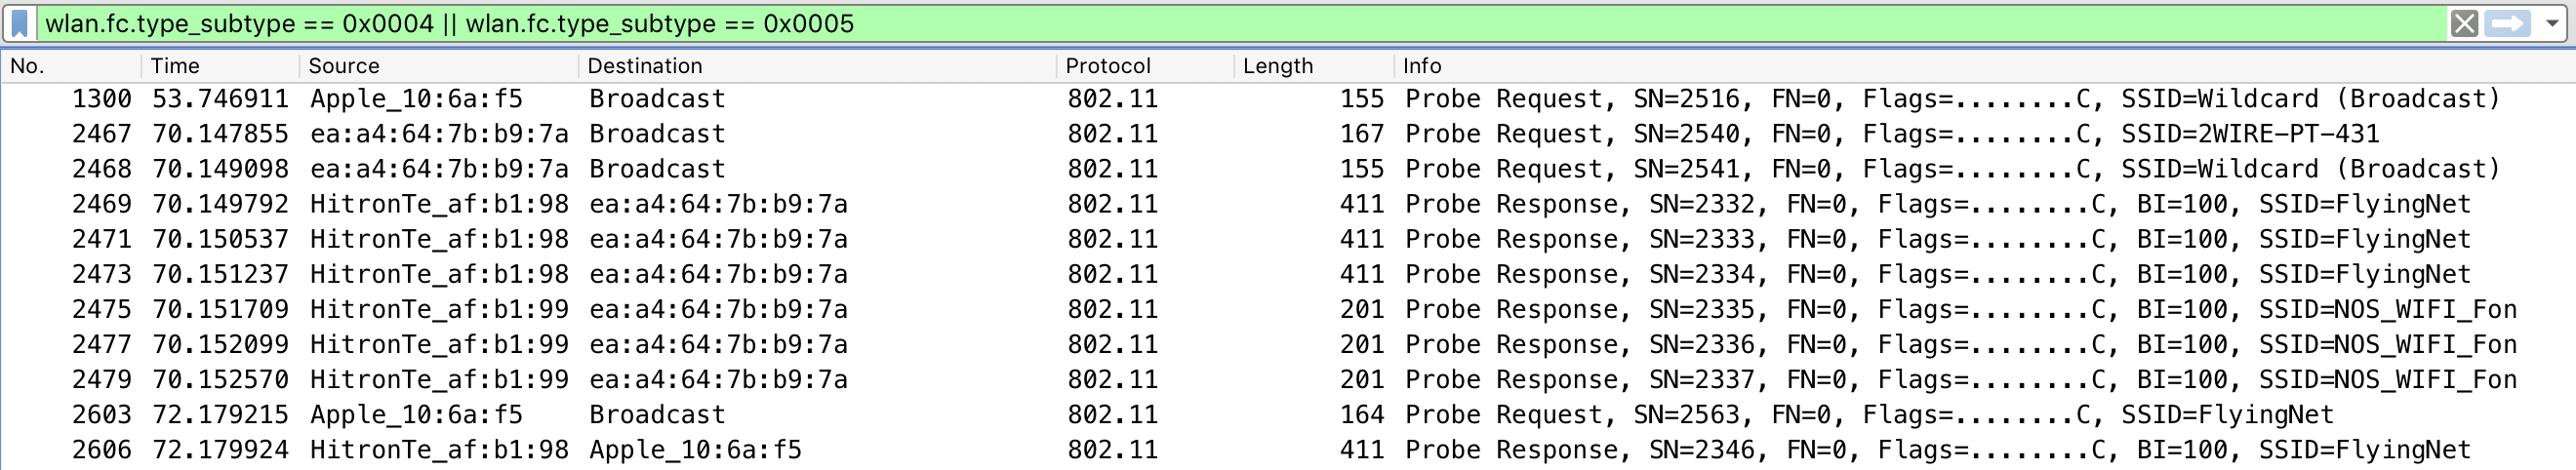
\includegraphics[scale=0.30]{10.png} 
\end{center}
\caption{\label{fig:10}Probing Requests e Probing Responses.}
\end{figure} 
\par
\textbf{R:} O filtro de visualização utilizado foi \textbf{wlan.fc.type\_subtype == 0x0004 || wlan.fc.type\_subtype == 0x0005}.


\subsection{Exercício 11}
\emph{Identifique um probing request para o qual tenha havido um probing response. Face ao endereçamento usado, indique a que sistemas são endereçadas estas tramas e explique qual o propósito das mesmas?}
\begin{figure}[H]
\begin{center}
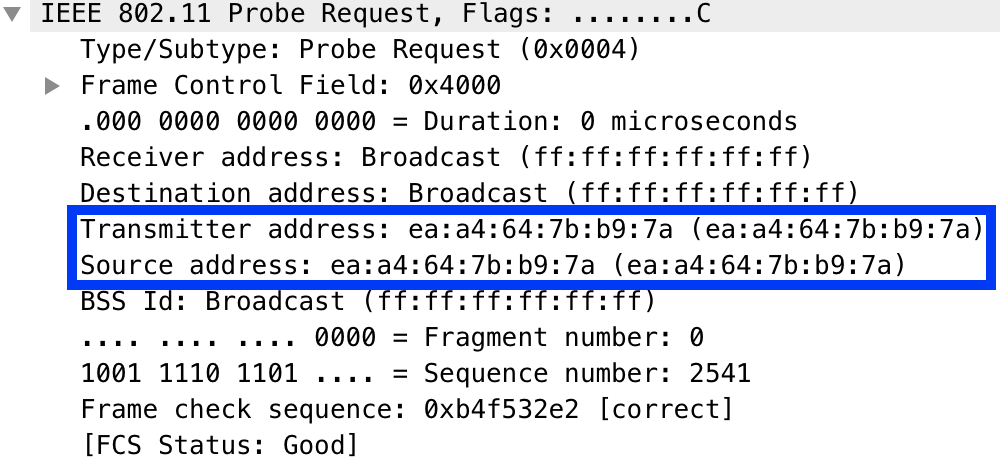
\includegraphics[scale=0.30]{11_Request.png} 
\end{center}
\caption{\label{fig:11_Request}Probe Request.}
\end{figure} 
\par
\begin{figure}[H]
\begin{center}
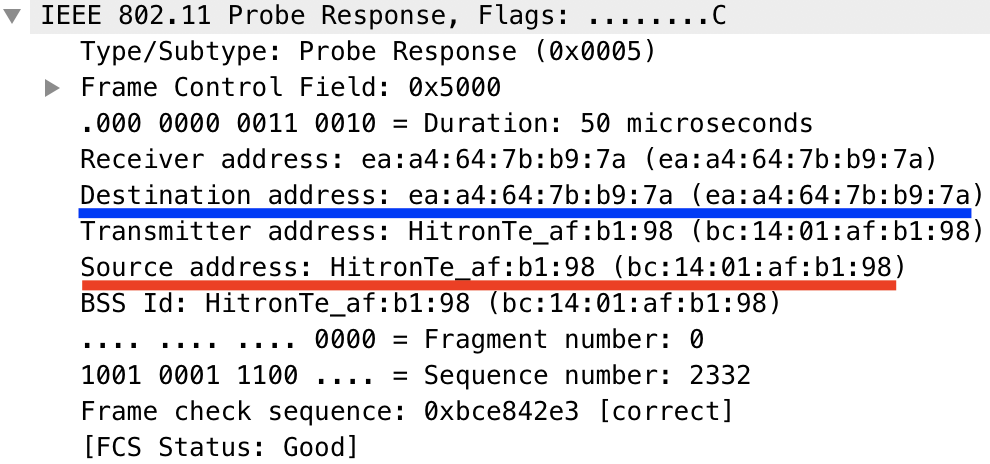
\includegraphics[scale=0.30]{11_Response.png} 
\end{center}
\caption{\label{fig:11_Response}Probe Response.}
\end{figure} 
\par
\textbf{R:} Como se pode verificar nas figuras \ref{fig:11_Request} e \ref{fig:11_Response}, inicialmente ocorreu um Probe Request proveniente de um aparelho com o endereço MAC \textbf{ea:a4:64:7b:b9:7a}, de seguida um AP com o endereço MAC \textbf{bc:14:01:af:b1:98} enviou um Probe Response de modo a poder dizer aparelho que se encontra disponível para que haja associação entre os dois.




\section{Processo de Associação}

\subsection{Exercício 12}
\emph{Identifique uma sequência de tramas que corresponda a um processo de associação completo entre a STA e o AP, incluindo a fase de autenticação.}
\begin{figure}[H]
\begin{center}
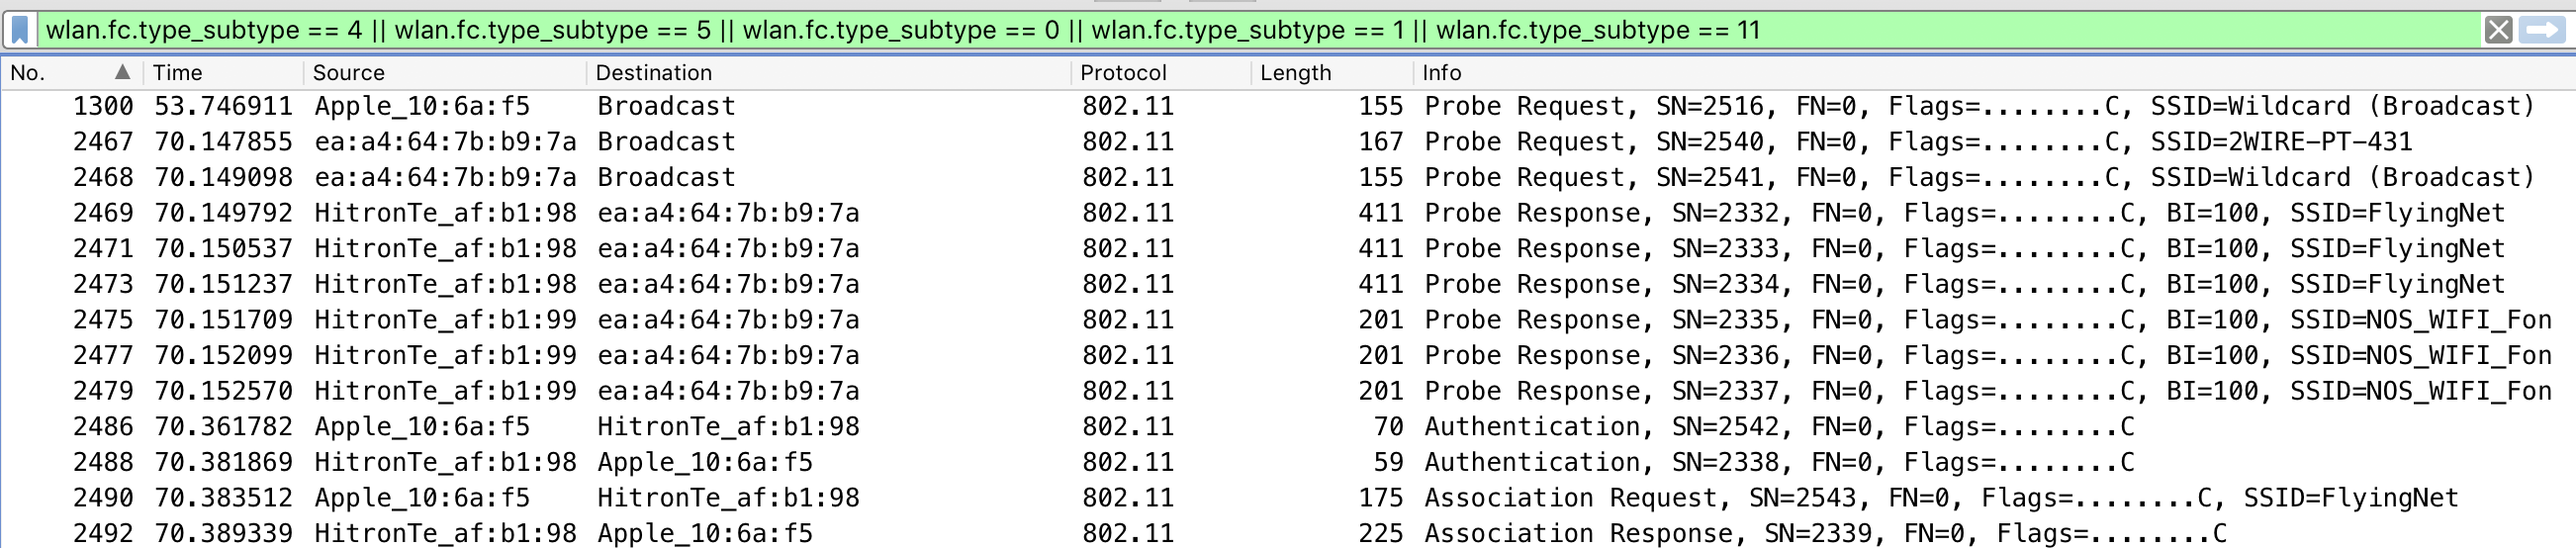
\includegraphics[scale=0.30]{12.png} 
\end{center}
\caption{\label{fig:12}Processo de associação.}
\end{figure} 
\par
\textbf{R:} 

O filtro de visualização utilizado foi \textbf{wlan.fc.type\_subtype == 4 || wlan.fc.type\_subtype == 5 ||wlan.fc.type\_subtype == 0 || wlan.fc.type\_subtype == 1 || wlan.fc.type\_subtype == 11}.

O processo de Scanning ativo ja foi identificado em questões anteriores. É então de grande importância referir as tramas de autenticação quem são respetivamente a trama \textbf{2486} e a trama \textbf{2488}, e as tramas de associação que são respetivamente a trama \textbf{2490} e a trama \textbf{2492}.


\subsection{Exercício 13}
\emph{Efetue um diagrama que ilustre a sequência de todas as tramas trocadas no processo.}

\textbf{R:}
\begin{figure}[H]
\begin{center}
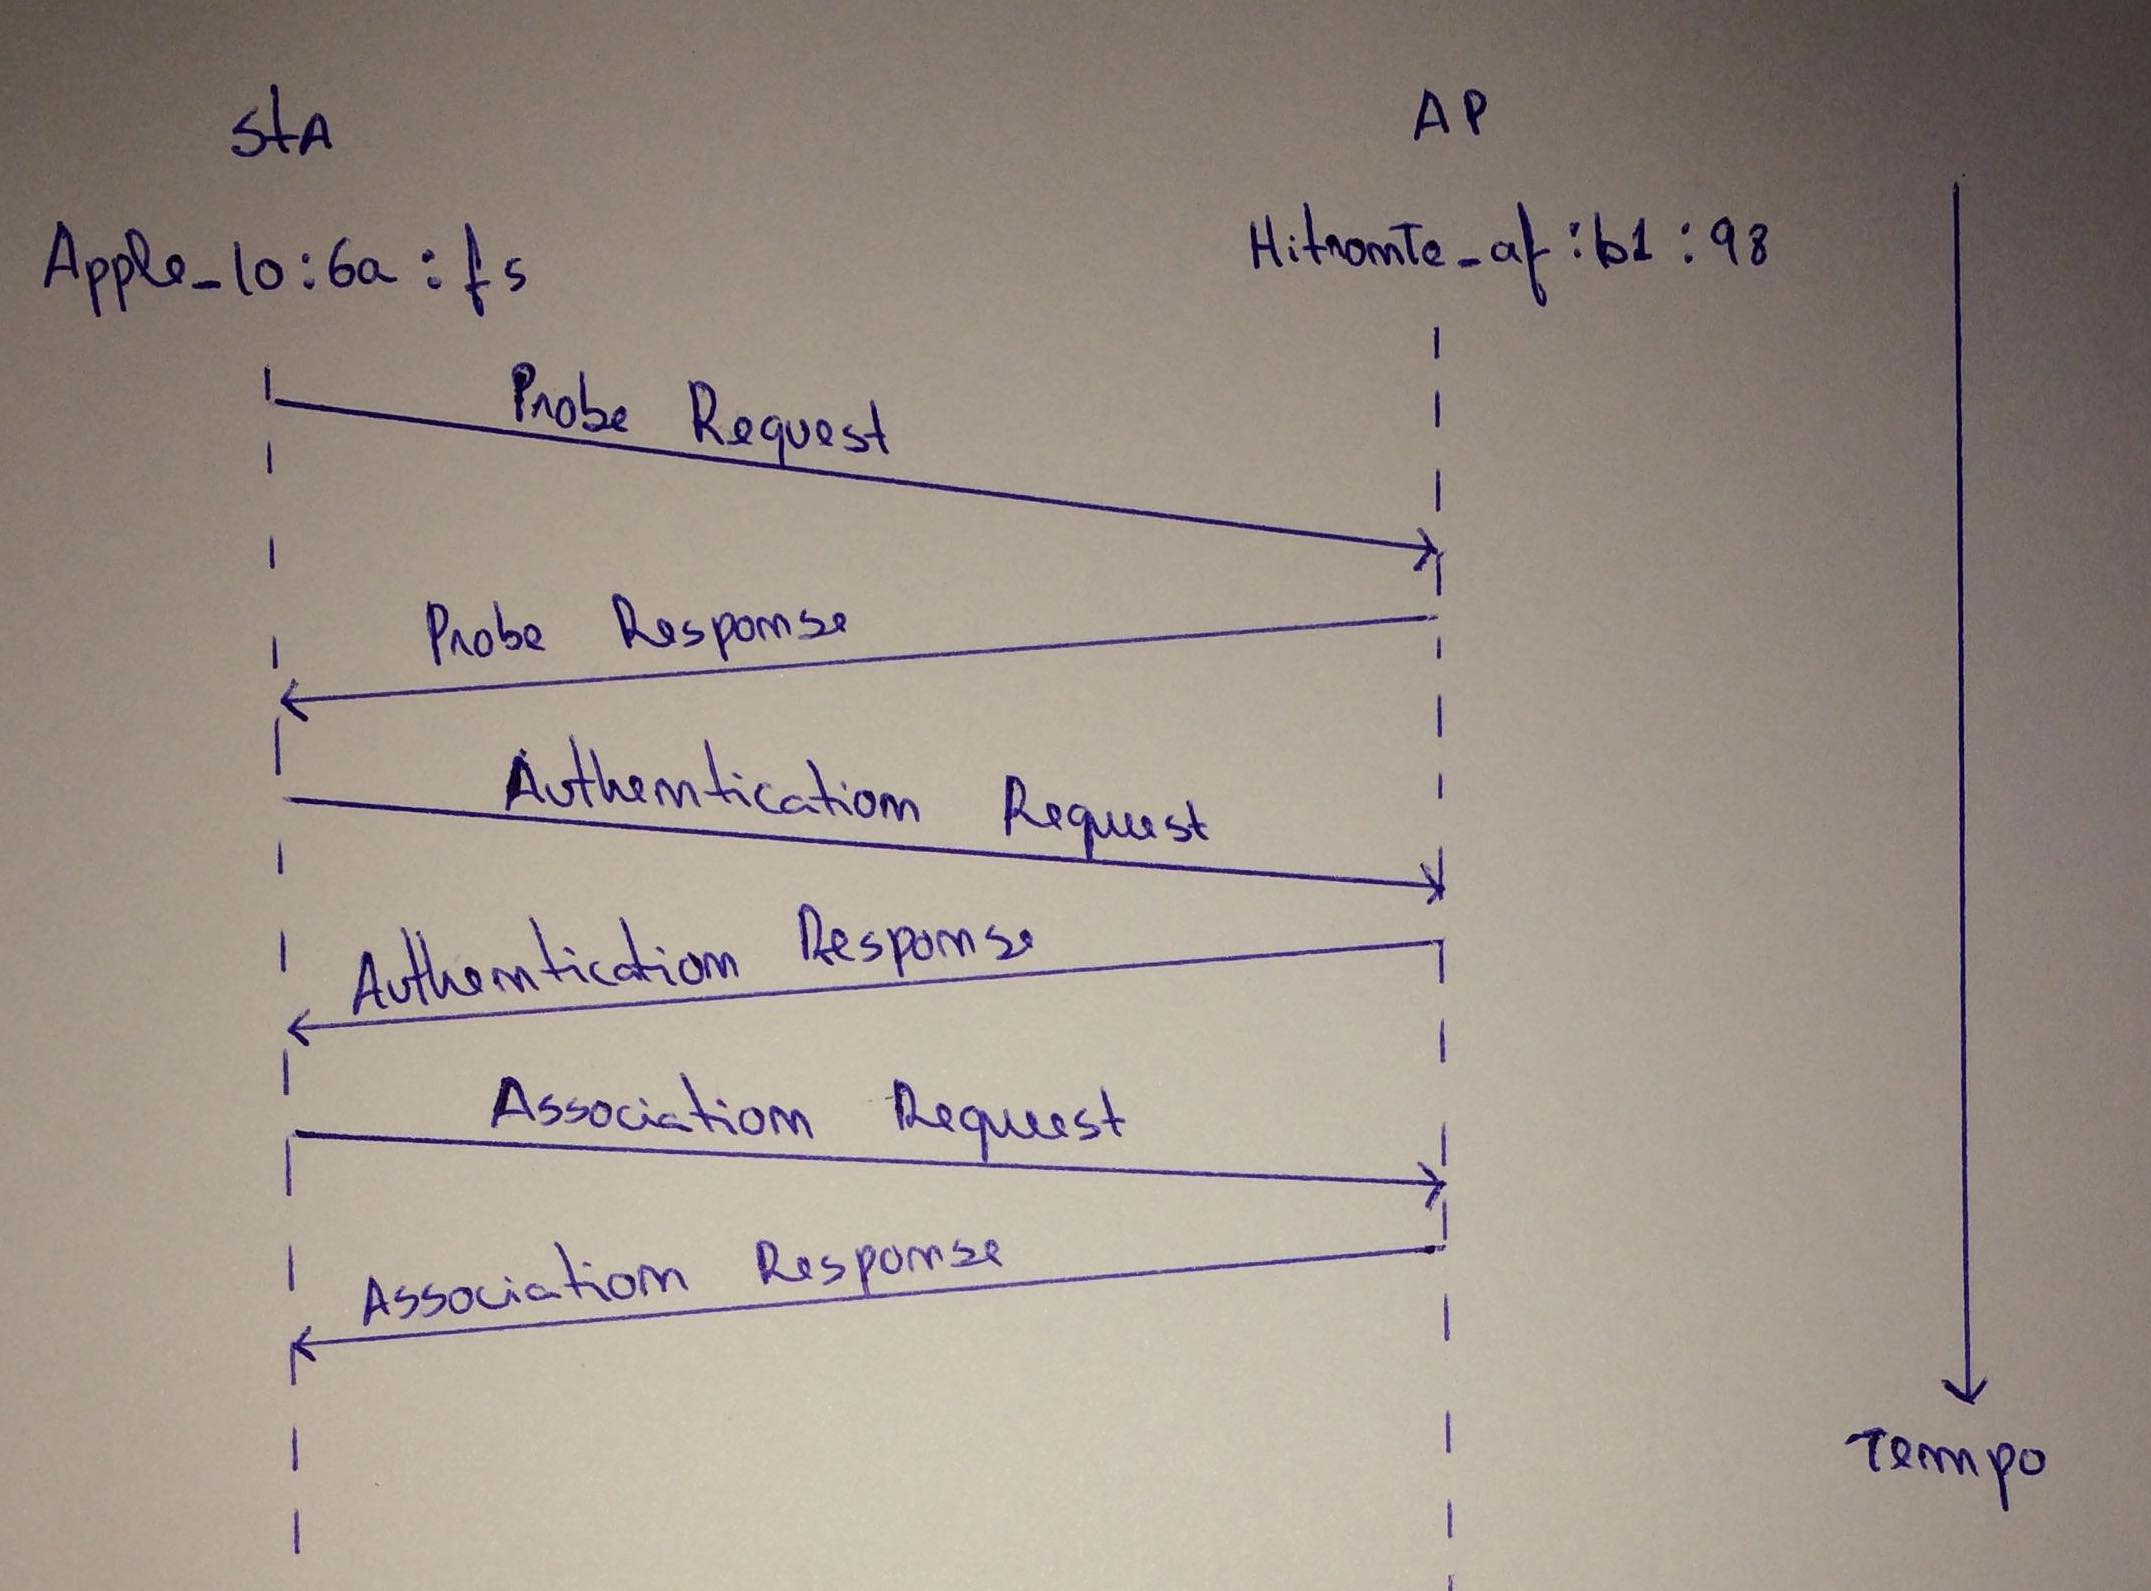
\includegraphics[scale=0.15]{13.png} 
\end{center}
\caption{\label{fig:13}Diagrama de tramas.}
\end{figure} 


\section{Transferência de Dados}

\subsection{Exercício 14}
\emph{Considere a trama de dados no455. Sabendo que o campo Frame Control contido no cabeçalho das tramas 802.11 permite especificar a direcionalidade das tramas, o que pode concluir face à direcionalidade dessa trama, será local à WLAN?}
\begin{figure}[H]
\begin{center}
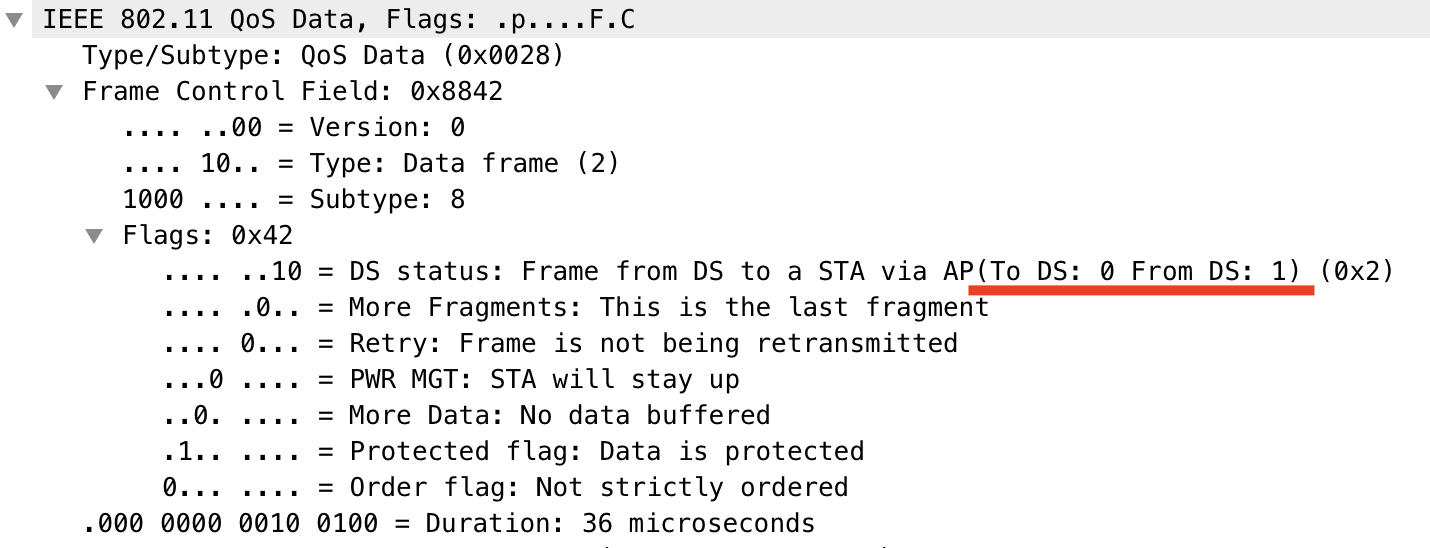
\includegraphics[scale=0.30]{14.png} 
\end{center}
\caption{\label{fig:14}Direcionalidade da trama 455.}
\end{figure} 
\par
\textbf{R:} Como se pode verificar na figura \ref{fig:14} sublinhado a vermelho, a direcionalidade da trama é \textbf{To DS: 0 From DS: 1}, o que significa que a trama é recebida pela station proveniente do sistema de distribuição via AP. A trama é local à WLAN.


\subsection{Exercício 15}
\emph{Para a trama de dados no455, transcreva os endereços MAC em uso, identificando qual o endereço MAC correspondente ao host sem fios (STA), ao AP e ao router de acesso ao sistema de distribuição?}
\begin{figure}[H]
\begin{center}
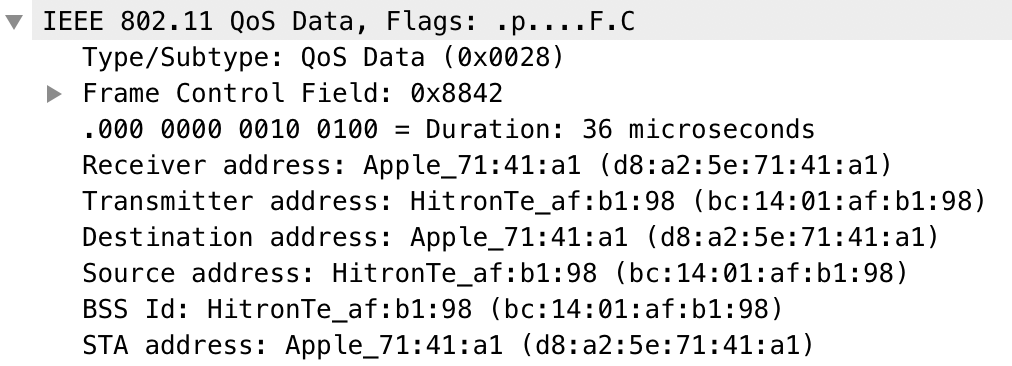
\includegraphics[scale=0.30]{15.png} 
\end{center}
\caption{\label{fig:15}Endereços da trama 455.}
\end{figure} 
\par
\textbf{R:} Como se pode verificar na figura \ref{fig:15}, o endereço MAC correspondente ao STA é \textbf{d8:a2:5e:71:41:a1}. Este corresponde também ao Receiver Address e ao Destination Address, visto estes identificarem o mesmo equipamento. O endereço MAC correspondente ao AP é o mesmo que o do router de acesso, apesar de estarem em campos da trama diferentes. Referimo-nos ao \textbf{bc:14:01:af:b1:98}. Este endereço MAC corresponde ao Source Address, ao Transmitter Address e ao BSSID.


\subsection{Exercício 16}
\emph{Como interpreta a trama no457 face à sua direccionalidade e endereçamento MAC?}
\begin{figure}[H]
\begin{center}
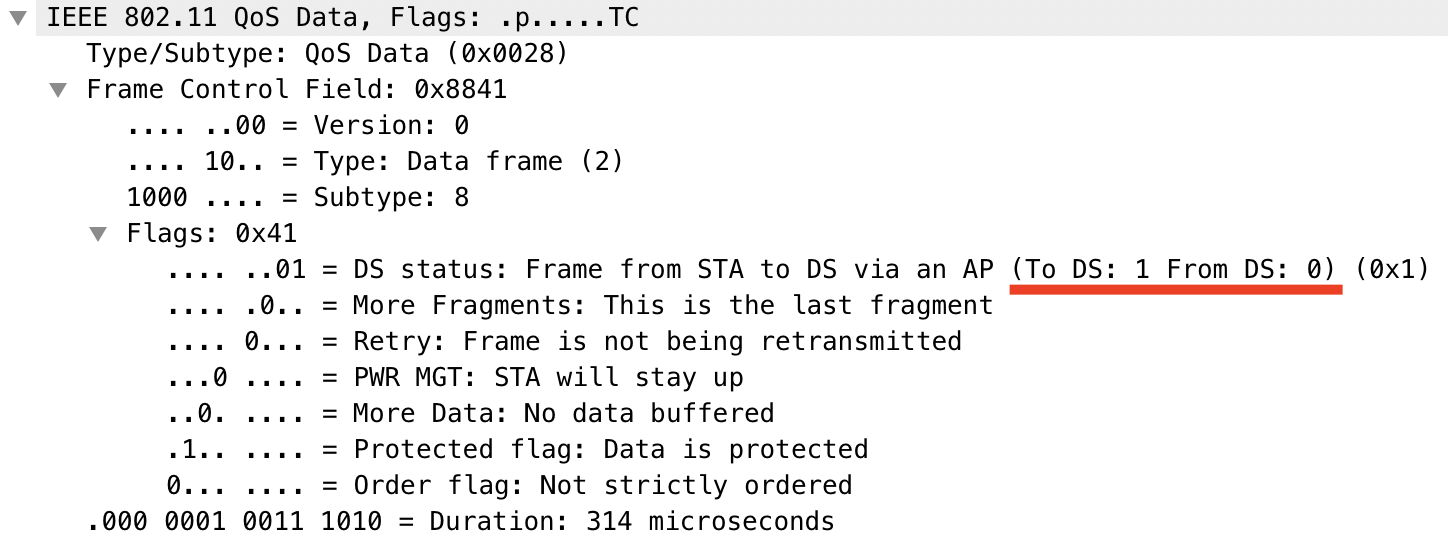
\includegraphics[scale=0.30]{16.png} 
\end{center}
\caption{\label{fig:16}Direcionalidade da trama 457.}
\end{figure} 

\begin{figure}[H]
\begin{center}
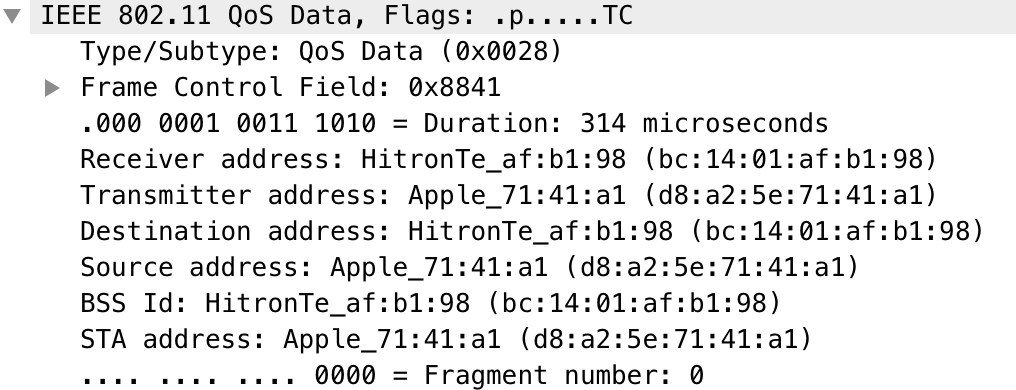
\includegraphics[scale=0.30]{16_2.png} 
\end{center}
\caption{\label{fig:16_2}Endereços da trama 457.}
\end{figure} 
\par
\textbf{R:} Como se pode verificar na figura \ref{fig:14} sublinhado a vermelho, a direcionalidade da trama é \textbf{To DS: 1 From DS: 0}, o que significa que a trama é enviada pela station para o sistema de distribuição via AP.

Quanto aos endereços MAC, estes são exatamente os opostos da trama 455 uma vez que a trama vai da estação para o AP e não do AP para a estação como se verificava na trama 455.


\subsection{Exercício 17}
\emph{Que subtipo de tramas de controlo são transmitidas ao longo da transferência de dados acima mencionada? Tente explicar porque razão têm de existir (contrariamente ao que acontece numa rede Ethernet).}
\\ \par
\textbf{R:} Os subtipos de tramas de controlo transmitidas são \textbf{Request-to-send},  \textbf{Clear-to-send} e \textbf{Acknowledgement}. Este tipo de tramas de controlo nas redes 802.11 têm de existir pois são a forma de lidar com as colisões que ocorrem através de estações escondidas, de uma forma geral este "protocolo" faz uma reserva de meio para poder transmitir.


\subsection{Exercício 18}
\emph{O uso de tramas Request To Send e Clear To Send, apesar de opcional, é comum para efetuar "pré-reserva" do acesso ao meio quando se pretende enviar tramas de dados, com o intuito de reduzir o número de colisões resultante maioritariamente de STAs escondidas. Para o exemplo acima, verifique se está a ser usada a opção RTS/CTS na troca de dados entre a STA e o AP/Router da WLAN, identificando a direccionalidade das tramas e os sistemas envolvidos.}
\begin{figure}[H]
\begin{center}
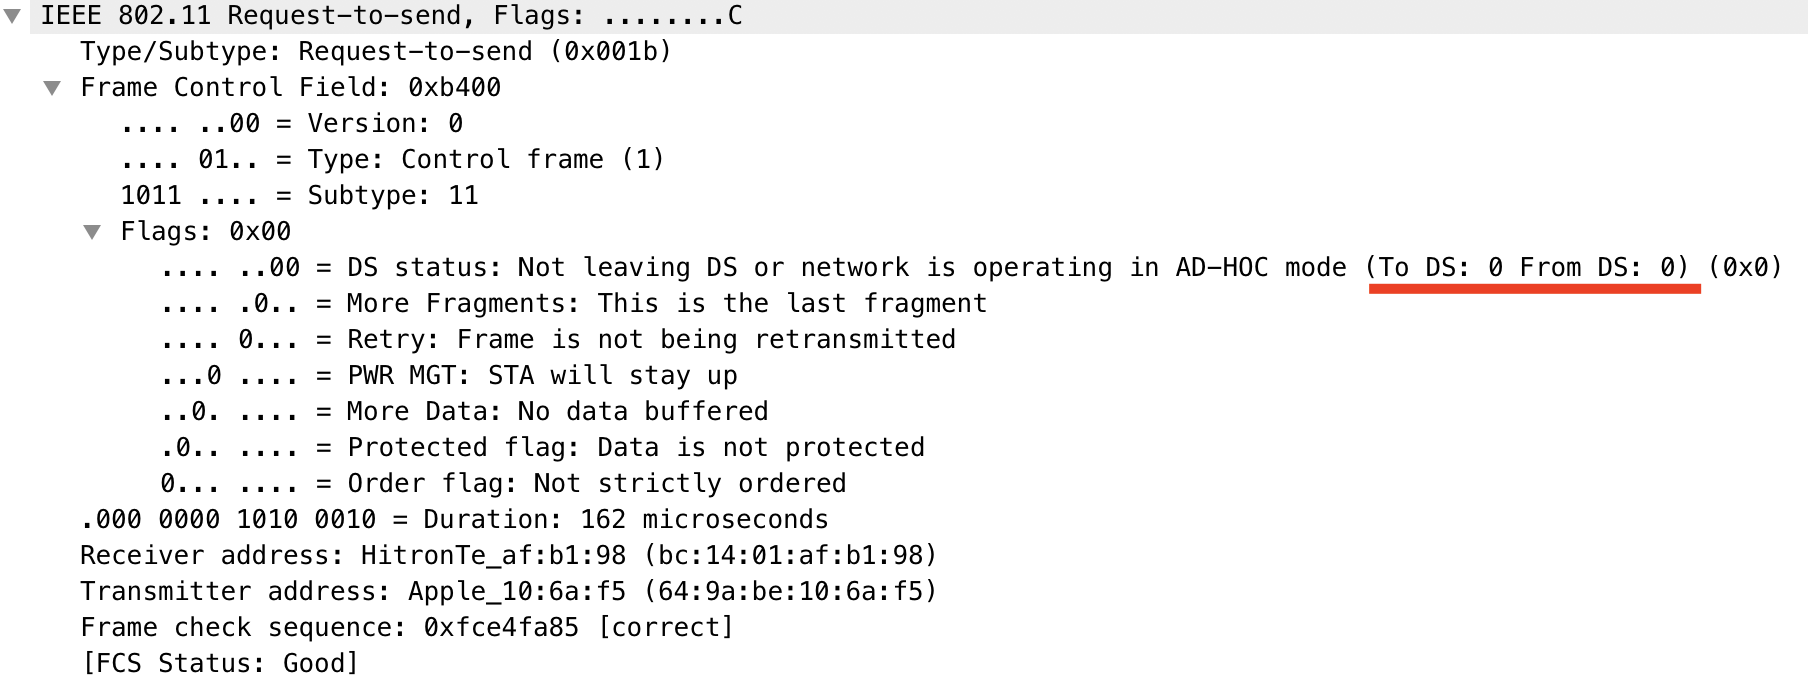
\includegraphics[scale=0.30]{18_RTS.png} 
\end{center}
\caption{\label{fig:18_RTS}Trama Request-to-Send.}
\end{figure} 

\begin{figure}[H]
\begin{center}
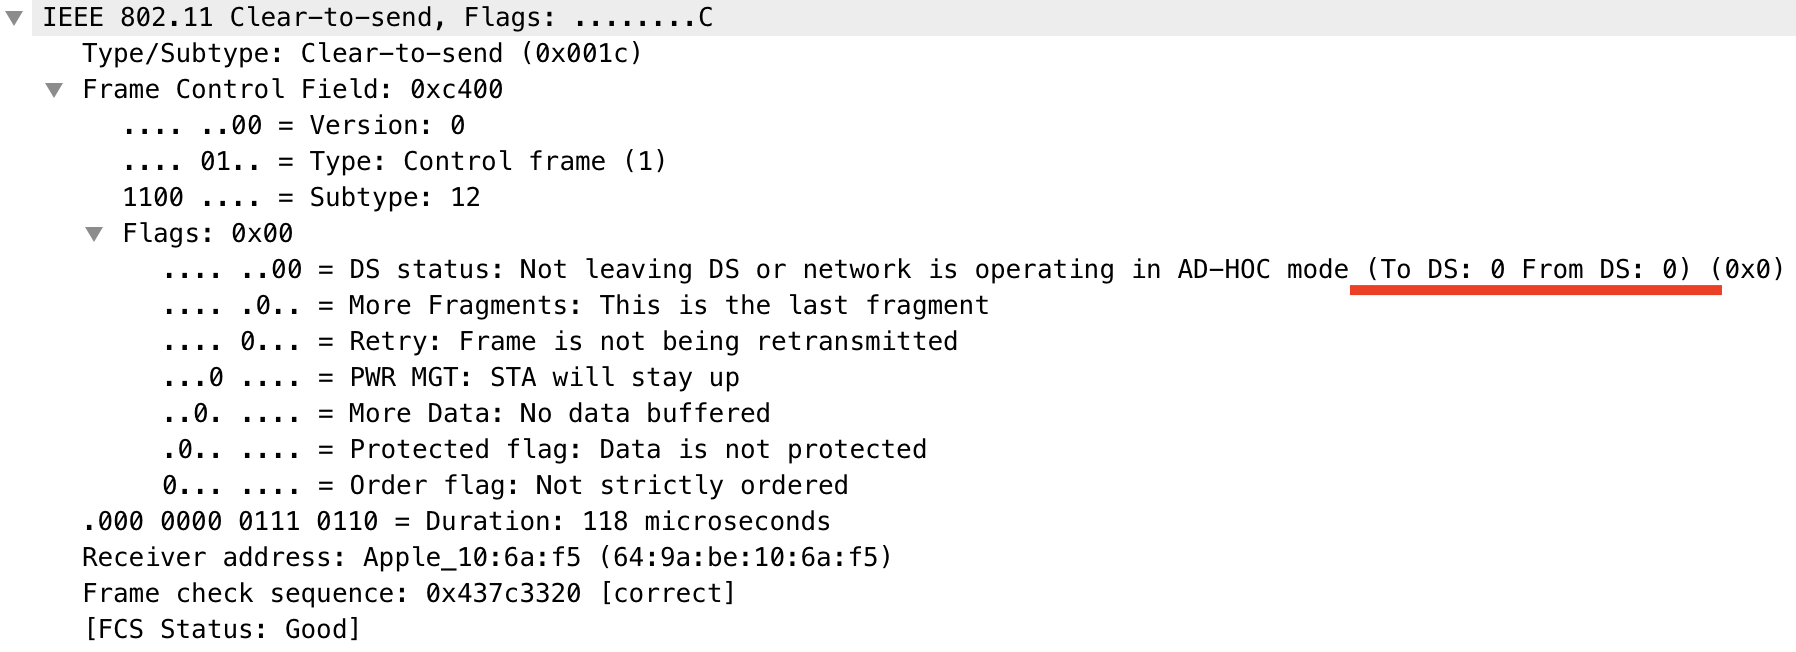
\includegraphics[scale=0.30]{18_CTS.png} 
\end{center}
\caption{\label{fig:18_CTS}Trama Clear-to-Send.}
\end{figure} 

\textbf{R:} Sim, estão a ser usadas tramas RTS/CTS. 

Primeiro a trama Request-to-Send é enviada da estação para o AP para tentar reservar o meio para transmitir, esta é feita em modo ad-hoc, uma vez que os campos ToDS e FromDS estão a 0, como é possível verificar na figura \ref{fig:18_RTS} sublinhado a vermelho.

O AP responde fazendo broadcast de uma trama Clear-to-Send, para avisar todas as estações quem pode transmitir. Esta trama é transmitida em modo ad-hoc uma vez que os campos ToDS e FromDS estão a 0, como é possível verificar na figura \ref{fig:18_CTS} sublinhado a vermelho.


\section{Conclusão}
Neste trabalho prático abordamos principalmente temas relacionados com Wireless e Redes Móveis.

Na primeira secção abordamos as frequências no qual as redes sem fios operam.

Na segunda e terceira secção trabalhamos com scanning ativo e passivo, nomeadamente as tramas beacon no primeiro caso, e os probing response e probing request no segundo caso.

Na quarta e última secção abordamos o endereçamento das tramas, com especial foco nas tramas de controlo.

Concluindo, com este guião exploramos a fundo as questões do nível de ligação de
dados em 802.11, e conseguimos de forma muito prática consolidar os conceitos mais teóricos do funcionamento
deste tipo de redes.

\end{document}